% Two versions: this file has the authors' credentials; main_blind.tex defines \blindversion
% and inputs this file to produce the double-blind version.
\newif\ifblind
\ifdefined\blindversion\blindtrue\fi
% Keep the current year as a number before ieeeaccess.cls turns \year into a macro (see below).
\edef\yearnum{\the\year}
\documentclass{ieeeaccess}
\usepackage{cite}
\usepackage{amsmath,amssymb,amsfonts}
\usepackage{graphicx}
\usepackage{textcomp}
\usepackage{booktabs}
\usepackage{array}
\usepackage{tabularx}
\usepackage{xcolor}
\usepackage{url}
% ieeeaccess.cls redefines \year as a macro; TikZ needs a number in \year while it loads,
% so lend it the real year and restore the class's version afterwards.
\let\accessyear\year
\let\year\yearnum
\usepackage{tikz}
\usetikzlibrary{positioning,arrows.meta,fit,backgrounds,patterns}
\usepackage{pgfplots}
\pgfplotsset{compat=newest}
\usepgfplotslibrary{groupplots}
% PANTONE 3015 C as process colour (the CMYK values ieeeaccess.cls gives it), so figures can use tints of the
% template blue. Every figure uses only this blue, its tints and grey.
\definecolor{pblue}{cmyk}{1,0.3,0,0.2}
\colorlet{pbluedark}{pblue!60!black}
% AQI category colours, exactly as AQI_COLORS in train.ipynb, for figures that show AirQo categories.
\definecolor{aqigood}{HTML}{2CA25F}\definecolor{aqimoderate}{HTML}{F1C40F}\definecolor{aqiusg}{HTML}{F39C12}
\definecolor{aqiunhealthy}{HTML}{E74C3C}\definecolor{aqivery}{HTML}{8E44AD}\definecolor{aqihazard}{HTML}{5B0F14}
\let\year\accessyear
% ieeeaccess.cls registers its PANTONE 3015 C spot colour in the page resources, and pgf/TikZ
% overwrites those resources at shipout, so viewers lose the colour (blank headings, captions).
% Register the colour space through pgf instead, so every page keeps it.
\makeatletter
\ifdefined\PANTONE
  \expandafter\pgfutil@addpdfresource@colorspaces\expandafter{\the\PANTONE}
\fi
\makeatother
% ieeeaccess captions read \xfigwd, which only its \Figure command sets; give TikZ figures a default.
\def\xfigwd{0pt}
% Subheadings: bold oblique, full black (the template's grey is faint) and 8 pt, one point below the 9 pt section headings.
\definecolor{greycolor}{cmyk}{0,0,0,1}
\def\sectionBfont{\sffamily\fontencoding{T1}\fontseries{b}\fontshape{sl}\fontsize{8}{11}\selectfont}
\usepackage[hidelinks]{hyperref}
\graphicspath{{figures/}}
\ifblind\hypersetup{pdfauthor={}}\else\hypersetup{pdfauthor={Charis Opol, Cole Rodney Migisha}}\fi

\newcommand{\aq}[1]{\textcolor{red}{[#1]}}
\newcommand{\ugm}{\textmu g/m\textsuperscript{3}}
\newcommand{\orcidicon}[1]{\href{#1}{\raisebox{-0.15ex}{
\includegraphics[height=1.25ex]{orcid-id.png}}}}
\def\BibTeX{{\rm B\kern-.05em{\sc i\kern-.025em b}\kern-.1667em\lower.7ex\hbox{E}\kern-.1257emX}}

\begin{document}

\newcommand{\papertitle}{Hourly PM\textsubscript{2.5} Prediction from Sparse Low-Cost Sensor Records in Ugandan Cities}
\title{\papertitle}
\ifblind
\author{Anonymous Authors\authorrefmark{1}}
\address[1]{Affiliation and contact details removed for double-blind review}
\else
% ORCID: Charis Opol https://orcid.org/0009-0003-7417-7984; Cole Rodney Migisha https://orcid.org/0009-0000-5311-2485
\author{Charis Opol\authorrefmark{1}\,\orcidicon{https://orcid.org/0009-0003-7417-7984}, Cole Rodney Migisha\authorrefmark{1}\,\orcidicon{https://orcid.org/0009-0000-5311-2485}}
\address[1]{Uganda Christian University, Mukono, Uganda, Faculty of Engineering, Design and Technology, Department of Computing and Technology  \\b29654@students.ucu.ac.ug \\b29657@students.ucu.ac.ug}
\fi

\begin{abstract}
Hourly PM\textsubscript{2.5} prediction from low-cost sensors is difficult when devices go offline and leave short, broken records. This paper evaluates hourly PM\textsubscript{2.5} prediction (one hour ahead when recent readings are used) from 14,600 hourly records of 149 AirQo and AirGradient sensors in Ugandan cities. We compared twelve models with mean and persistence baselines under three validation designs, and tested them without retraining on a later full month. A first model reached a mean absolute error (MAE) of 3.10~\ugm{} only because it was given PM\textsubscript{10}, a same-hour co-measurement. Without PM\textsubscript{10}, a support vector regressor cut the mean baseline's MAE by 47\% but gained only 5\% in August. With three hours of PM\textsubscript{2.5} history, tree models matched persistence on the hold-out (8.43 against 8.58~\ugm{}) and beat it by 10\% in August. Better imputation filled gaps well without improving prediction. In sparse networks, the last reading matters more than weather inputs.
\end{abstract}

\begin{keywords}
PM\textsubscript{2.5} forecasting, Low-cost sensors, AirQo, Missing-data imputation, Time-series validation, Model deployment
\end{keywords}

\titlepgskip=-15pt
\maketitle

\section{Introduction}

Fine particulate matter (PM2.5) is the pollutant of greatest health concern in most cities; the World Health Organization's annual guideline for it is 5~\ugm{}~\cite{ref01}. In Kampala, an estimated 7,257 deaths between 2018 and 2021, about 18--20\% of all deaths each year, were attributable to exposure above that guideline~\cite{ref21}, and PM2.5 data serve Sustainable Development Goal indicators 3.9.1 and 11.6.2~\cite{ref22,ref23}. In Uganda, the AirQo network fills gaps between costly reference monitors with low-cost optical sensors~\cite{ref02,ref03}, whose readings need calibration~\cite{ref04}, diverge at high concentrations~\cite{ref05} and stop when devices go offline: AirQo devices reported in about 72\% of expected hours in April-June 2025~\cite{ref_sserunjogi2025}.

The forecasting study we reviewed in full used two years of data~\cite{ref06}; a new or intermittent network may have far less. Our file, labelled January to July 2026, holds readings on only eight days. We ask how much hourly PM2.5 skill such a record supports, and whether it holds in a later month, and report the rebuilt pipeline, its deployment and the alternatives we rejected.

\subsection{Objectives}\label{sec:objectives}

\textbf{Main objective.} To establish how much hourly PM2.5 prediction skill a sparse record of low-cost sensor readings supports, and whether a model built on it can be put to practical use. \textbf{Specific objectives:}

\begin{enumerate}
\item to quantify the skill that weather, time and sensor identity alone support;
\item to assess how much three hours of recent PM2.5 history add;
\item to evaluate whether more accurate filling of missing weather data improves predictions;
\item to assess how stable the results are across three validation designs and on a later month; and
\item to demonstrate that the model can be served on free cloud tiers, and report the constraints met.
\end{enumerate}

To our knowledge, no study we examined asks what a record of a few days supports. We contribute a comparison with mean and persistence baselines (Objectives 1--2), a test of whether better imputation helps (Objective 3), a transfer test on an unseen month (Objective 4) and a measured free deployment (Objective 5).

\section{Related Work}\label{sec:related}

Okure et al.~\cite{ref02} characterised air quality in Ugandan towns with AirQo sensors, and Sserunjogi et al.~\cite{ref03} published hourly data from 68 AirQo stations. Calibration cut RMSE from 18.6 to 7.2~\ugm{} for AirQo sensors~\cite{ref04} and from 20.37 to 3.83~\ugm{} in South Central Uganda~\cite{ref24}, but sensors still dispersed from a reference monitor at high concentrations~\cite{ref05}.

Weather is the usual input, but its effect varies with place and season~\cite{ref07,ref08}; Wabinyai et al.~\cite{ref09} modelled daily PM2.5 in Kampala from meteorology and lagged pollution. How could a record of a few days sample such effects?

Febrian and Permai~\cite{ref06} found past pollutants alone sufficient for seven-day forecasts in Jakarta, and Niyonzima et al.~\cite{ref10} forecast PM2.5 one hour ahead on a large AirQo record. Work on sparse networks borrows from elsewhere: Rwandan sensors~\cite{ref25}, Gaussian processes over AirQo sites~\cite{ref26}, a graph network over 511 sensors in Bihar~\cite{ref27} and transfer from data-rich regions~\cite{ref28}. We ask what a sensor's own few days support.

\section{Methodology}\label{sec:method}

Fig.~\ref{fig:pipeline} shows the training path, described here, and the deployed path, described in Section~\ref{sec:technology}.

\begin{figure}[t]
\centering
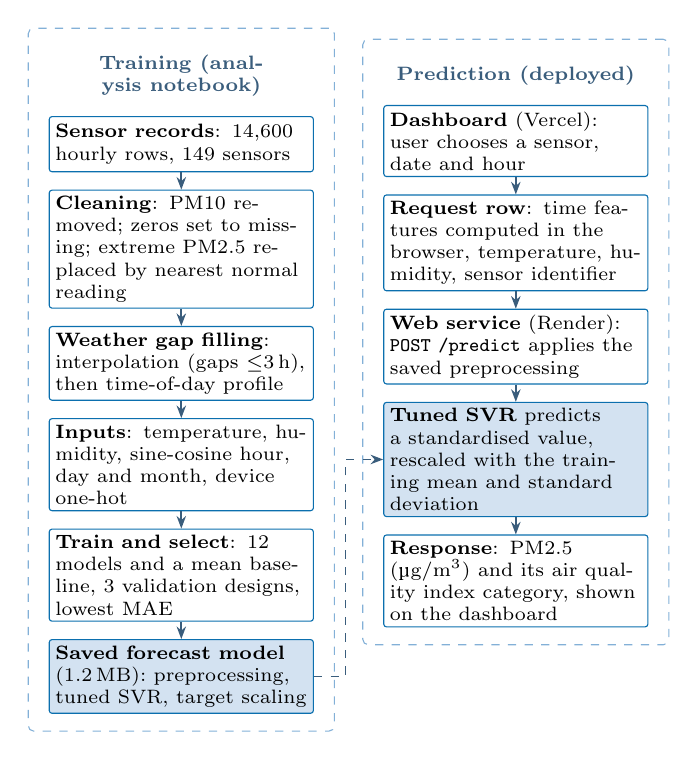
\begin{tikzpicture}[
  font=\scriptsize,
  node distance=2.2mm,
  box/.style={draw=pblue, rounded corners=1pt, align=left, inner sep=2.2pt,
               text width=32mm, minimum height=7mm, fill=white},
  lane/.style={draw=pblue!45, dashed, rounded corners=2pt, inner sep=2.2mm},
  lanetitle/.style={font=\scriptsize\bfseries, text=pbluedark, align=center, text width=32mm},
  flow/.style={-{Stealth[length=1.6mm]}, semithick, draw=pbluedark},
]
% Training lane (notebook, offline)
\node[lanetitle] (tt) {Training (analysis notebook)};
\node[box, below=1.2mm of tt] (t1) {\textbf{Sensor records}: 14,600 hourly rows, 149 sensors};
\node[box, below=of t1] (t2) {\textbf{Cleaning}: PM10 removed; zeros set to missing; extreme PM2.5 replaced by nearest normal reading};
\node[box, below=of t2] (t3) {\textbf{Weather gap filling}: interpolation (gaps $\le$3\,h), then time-of-day profile};
\node[box, below=of t3] (t4) {\textbf{Inputs}: temperature, humidity, sine-cosine hour, day and month, device one-hot};
\node[box, below=of t4] (t5) {\textbf{Train and select}: 12 models and a mean baseline, 3 validation designs, lowest MAE};
\node[box, below=of t5, fill=pblue!15] (t6) {\textbf{Saved forecast model} (1.2\,MB): preprocessing, tuned SVR, target scaling};
\foreach \a/\b in {t1/t2,t2/t3,t3/t4,t4/t5,t5/t6} \draw[flow] (\a) -- (\b);

% Prediction lane (deployed, online)
\node[lanetitle, right=8mm of tt] (pt) {Prediction (deployed)};
\node[box, below=1.2mm of pt] (p1) {\textbf{Dashboard} (Vercel): user chooses a sensor, date and hour};
\node[box, below=of p1] (p2) {\textbf{Request row}: time features computed in the browser, temperature, humidity, sensor identifier};
\node[box, below=of p2] (p3) {\textbf{Web service} (Render): \texttt{POST /predict} applies the saved preprocessing};
\node[box, below=of p3, fill=pblue!15] (p4) {\textbf{Tuned SVR} predicts a standardised value, rescaled with the training mean and standard deviation};
\node[box, below=of p4] (p5) {\textbf{Response}: PM2.5 (\ugm) and its air quality index category, shown on the dashboard};
\foreach \a/\b in {p1/p2,p2/p3,p3/p4,p4/p5} \draw[flow] (\a) -- (\b);

\begin{scope}[on background layer]
  \node[lane, fit=(tt)(t1)(t6)] (L) {};
  \node[lane, fit=(pt)(p1)(p5)] (R) {};
\end{scope}
% the saved model is loaded by the service
\draw[flow, dashed] (t6.east) -- ++(4mm,0) |- (p4.west);
\end{tikzpicture}
\caption{The training path (left) and one prediction request (right). Models with PM2.5 history are not served.}
\label{fig:pipeline}
\end{figure}

\subsection{Data}\label{sec:data}

Both files are hourly exports from the AirQo network, which also reports AirGradient devices~\cite{ref29}, obtained in September and October 2026. AirQo licenses its data under CC BY 4.0 and asks users to credit it and the originating provider and to treat readings as indicative~\cite{ref_airqo_terms}; we credit AirQo and AirGradient here. The main file holds 14,600 hourly records of temperature, humidity and calibrated PM2.5 and PM10 from 149 devices, 143 with coordinates (Fig.~\ref{fig:map}), but only on 1--3 January, 1--2 April and 1--3 June 2026, 147 hours in all (Fig.~\ref{fig:eda}). About 28.8\% of AirQo rows report 0~\textdegree{}C and 0\% humidity together (weather dropouts), and in 22.6\% of rows reporting both pollutants PM2.5 exceeded PM10, a sign of calibration error. The August file (73,274 rows, 125 of the same sensors, mean 35.5~\ugm{}) served only as an external test.

\begin{figure*}[t]
\centering
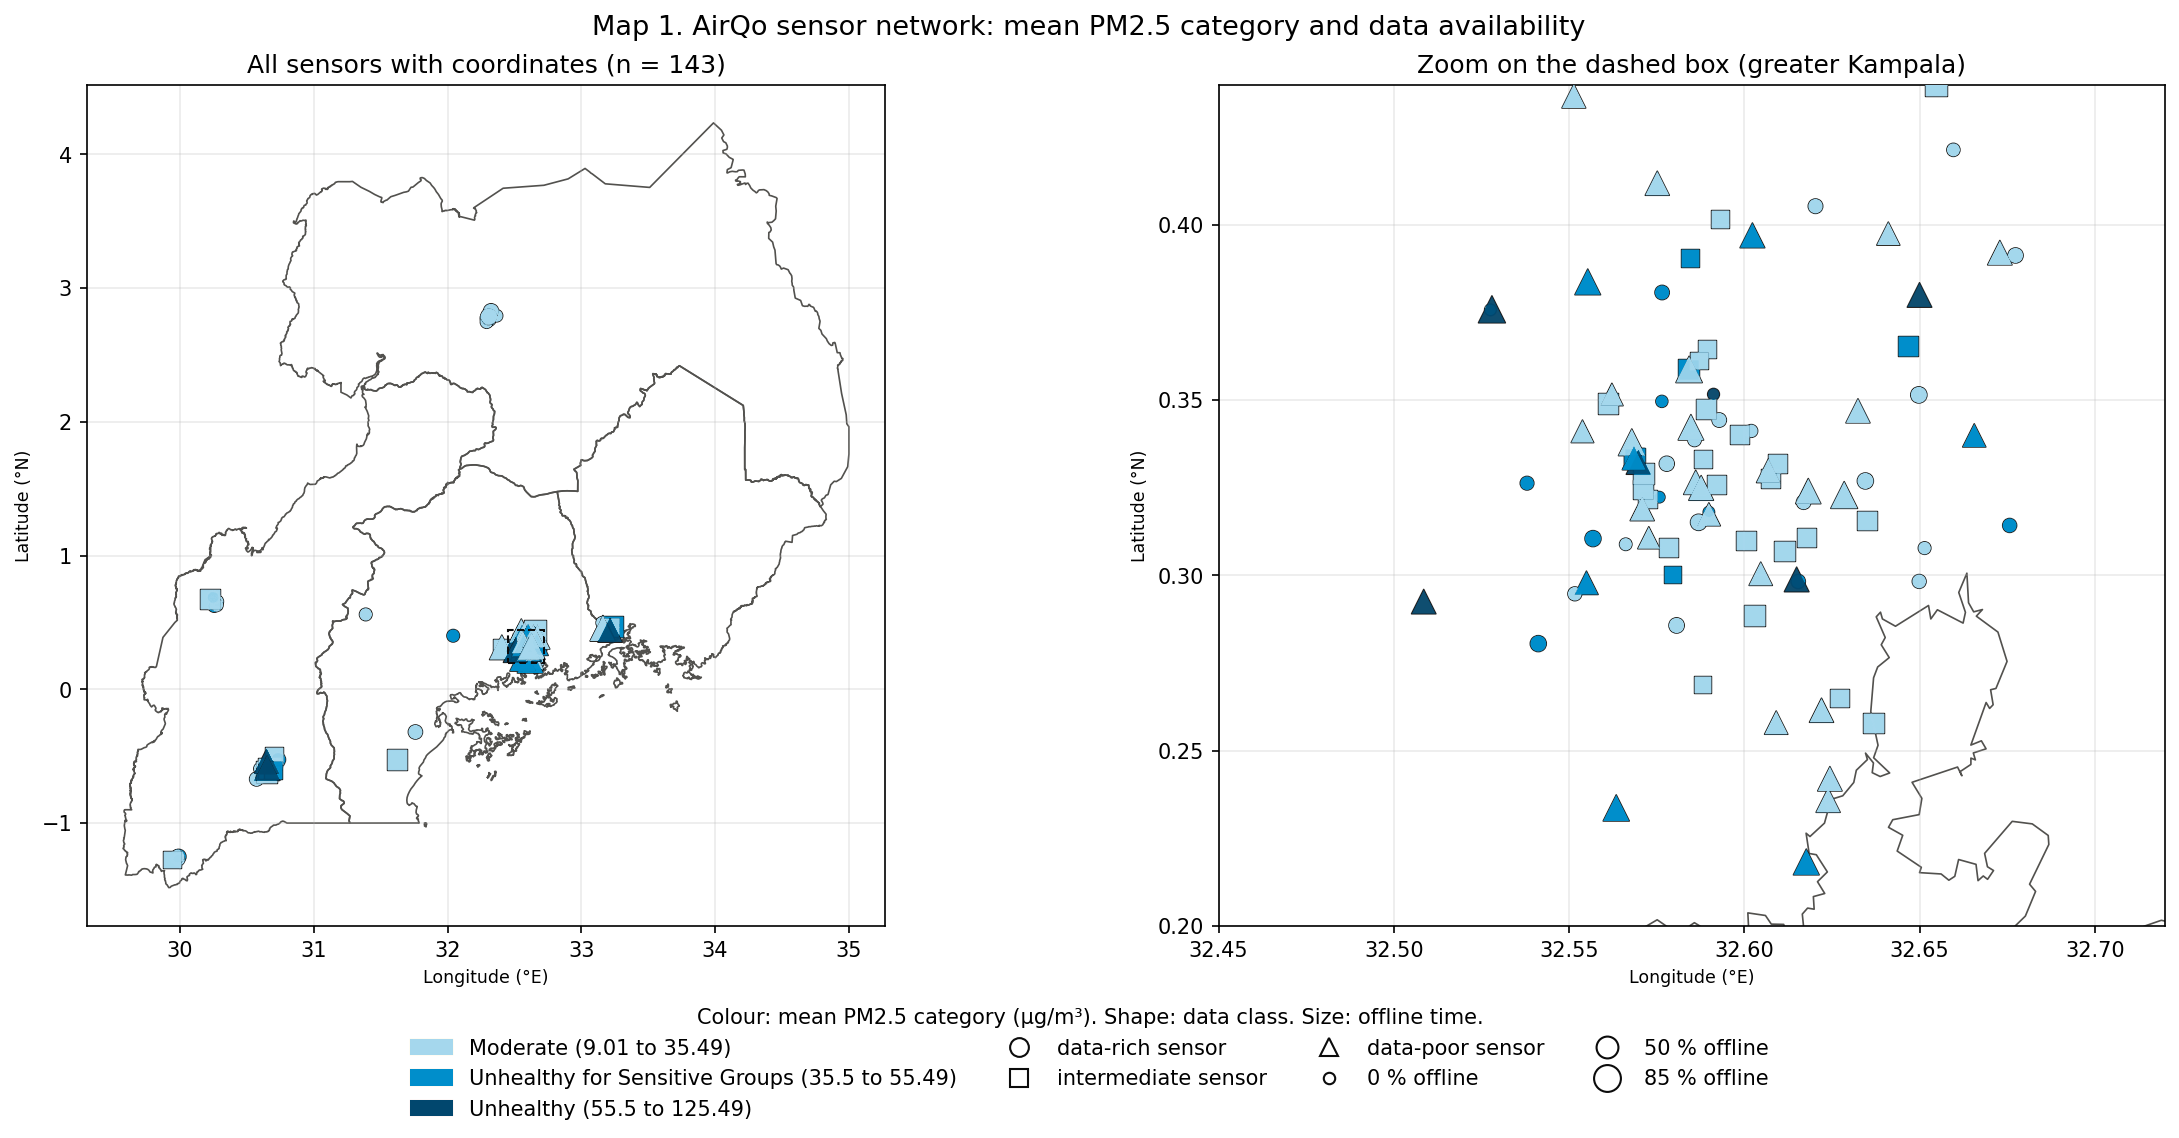
\includegraphics[width=0.82\textwidth]{map_sensor_network.png}
\caption{The AirQo sensors that report coordinates (n = 143), coloured by mean PM2.5 category; marker shape gives data availability and size the share of time offline. Right: greater Kampala.}
\label{fig:map}
\end{figure*}

\begin{figure*}[t]
\centering
% Generated by research_paper_draft3/reruns/make_figures_tex.py from review_extras (train.ipynb rerun).
\begin{tikzpicture}
\begin{groupplot}[group style={group size=2 by 2, horizontal sep=10mm, vertical sep=14mm},
  width=0.5\textwidth, height=38mm, xmin=-0.5, xmax=146.5, ymin=0, ymax=185,
  xtick={0,49,95}, xticklabels={1 Jan,1 Apr,1 Jun},
  xlabel={Observation hours, in three bursts}, ylabel={PM2.5 (\ugm)}, label style={font=\scriptsize}, tick label style={font=\scriptsize},
  title style={font=\scriptsize\bfseries, text=pbluedark}, ymajorgrids, grid style={black!15},
  axis x line*=bottom, axis y line*=left, unbounded coords=jump]
\nextgroupplot[title={Sensor airqo\_g5282: data-rich, 0\% offline}]
\addplot[black!40, line width=0.5pt, densely dashed] table[x=h, y=pm25_raw, col sep=comma] {figures/data/fig_eda_1.csv};
\addplot[pbluedark, line width=0.8pt] table[x=h, y=pm25, col sep=comma] {figures/data/fig_eda_1.csv};
\draw[black!35, densely dotted] (axis cs:48.5,0) -- (axis cs:48.5,185);\draw[black!35, densely dotted] (axis cs:94.5,0) -- (axis cs:94.5,185);
\nextgroupplot[title={Sensor aq\_04: data-poor, 82\% offline}]
\addplot[black!40, line width=0.5pt, densely dashed] table[x=h, y=pm25_raw, col sep=comma] {figures/data/fig_eda_2.csv};
\addplot[pbluedark, line width=0.8pt] table[x=h, y=pm25, col sep=comma] {figures/data/fig_eda_2.csv};
\draw[black!35, densely dotted] (axis cs:48.5,0) -- (axis cs:48.5,185);\draw[black!35, densely dotted] (axis cs:94.5,0) -- (axis cs:94.5,185);
\nextgroupplot[title={Sensor airqo\_g5566: data-poor, 73\% offline}]
\addplot[black!40, line width=0.5pt, densely dashed] table[x=h, y=pm25_raw, col sep=comma] {figures/data/fig_eda_3.csv};
\addplot[pbluedark, line width=0.8pt] table[x=h, y=pm25, col sep=comma] {figures/data/fig_eda_3.csv};
\draw[black!35, densely dotted] (axis cs:48.5,0) -- (axis cs:48.5,185);\draw[black!35, densely dotted] (axis cs:94.5,0) -- (axis cs:94.5,185);
\nextgroupplot[title={Sensor airqo\_g5551: data-poor, 69\% offline}]
\addplot[black!40, line width=0.5pt, densely dashed] table[x=h, y=pm25_raw, col sep=comma] {figures/data/fig_eda_4.csv};
\addplot[pbluedark, line width=0.8pt] table[x=h, y=pm25, col sep=comma] {figures/data/fig_eda_4.csv};
\draw[black!35, densely dotted] (axis cs:48.5,0) -- (axis cs:48.5,185);\draw[black!35, densely dotted] (axis cs:94.5,0) -- (axis cs:94.5,185);
\end{groupplot}
\end{tikzpicture}

\caption{Hourly PM2.5 at a data-rich and three data-poor sensors over the 147 hours with readings (solid: cleaned; dashed: untouched readings; dotted: burst boundaries).}
\label{fig:eda}
\end{figure*}

\subsection{Preparation and Imputation}\label{sec:preparation-and-imputation}

PM10 was removed, because same-hour PM10 contains the PM2.5 fraction and would leak the target; other AirQo studies also model PM2.5 without it~\cite{ref26,ref35}. Zeros were set to missing. A PM2.5 reading above its sensor's third quartile plus three interquartile ranges (Tukey's far-out limit~\cite{ref36}) was replaced by the sensor's nearest normal reading within six hours, as removing outliers improved AirQo forecasts in~\cite{ref26}. This changed 225 of 14,275 readings (1.5\%); since 52\% coincided with extremes at three or more other sensors, some may have been real episodes, so the untouched readings were kept for scoring. Missing PM2.5 targets were never imputed, and rows with PM2.5 above PM10 were kept, because the excess was usually small (median 4.2~\ugm{}).

Missing temperature and humidity were filled by (a) windowed interpolation across gaps of at most three hours, (b) a time-of-day profile per sensor with a local offset, or (c) a BRITS-style bidirectional LSTM~\cite{ref11,ref12}; all were fitted on training data only, and the final models used (a) then (b). Inputs are temperature, humidity, hour, day of week and month (as sine-cosine pairs) and a device code. Forecast models use only these, so they can predict any hour; nowcast models add the sensor's PM2.5 one to three hours earlier, so they need live readings.

\subsection{Models and Validation}\label{sec:models-and-validation}

Twelve models (Table~\ref{tab:models}) were compared with two baselines: the training mean, and persistence, which repeats each sensor's last reading within three hours. Hyperparameters were tuned with time-ordered cross-validation in scikit-learn~\cite{ref19}; the LSTMs had 32 units and dropout of 0.2; SMOTE for regression~\cite{ref13,ref14} was tested at strengths of 0.25 and 0.5; and one random seed (42) was fixed.

Models were scored on a chronological hold-out (train to 1 June, 11,633 rows; test 2--3 June, 2,642 rows), expanding-window cross-validation (test on 1 April, 2 April and 1 June in turn), leave-sensors-out validation (three folds of about 50 sensors) and August, by MAE with RMSE and $R^2$. 95\% confidence intervals come from 1,000 bootstrap resamples of sensors, since hours of one sensor are not independent. Imputation was tested on hidden readings in gaps of 1--24 hours and downstream by retraining five models; Evidently~\cite{ref20} measured drift and SHAP~\cite{ref15,ref16} attributions.

\begin{table}[t]
\caption{Models, inputs and final settings. W: weather; T: hour, weekday and month; S: sensor; H: PM2.5 one to three hours earlier.}
\label{tab:models}
\centering
\footnotesize
\begin{tabularx}{\columnwidth}{>{\raggedright\arraybackslash}X>{\raggedright\arraybackslash}X>{\raggedright\arraybackslash}X}
\toprule
Model & Inputs & Final settings \\
\midrule
Training mean; persistence & none; last reading within 3 h & - \\
Linear; polynomial; ridge regression & W, T, S & no intercept; degree 1; alpha 100 \\
Random forest, untuned; tuned~\cite{ref17} & W, T, S & 200 trees; 100 trees; min. leaf 2 \\
SVR & W, T, S & RBF kernel, C 5, epsilon 0.05 \\
KNN & W, T, S & 5 neighbours, Manhattan distance \\
LightGBM~\cite{ref18} & W, T, S & 800 trees, learning rate 0.05, 31 leaves \\
LSTM & W, T as 6-h sequence & see text \\
Random forest + history & W, T, S, H & 200 trees, min. leaf 2 \\
LightGBM + history & W, T, S, H & 200 trees, learning rate 0.1, 31 leaves \\
LSTM + history & W, T, previous-hour PM2.5 & see text \\
\bottomrule
\end{tabularx}
\end{table}

\section{Technology Description}\label{sec:technology}

\subsection{Design Tools}\label{sec:design-tools}

Table~\ref{tab:tools} lists the tools. The pipeline is one Jupyter notebook (about 56 minutes on a laptop without a GPU); the forecast model is saved with its preprocessing as one 1.2 MB file, which a standalone script reproduced exactly on all 2,642 test rows.

\begin{table}[t]
\caption{Design tools and their purpose.}
\label{tab:tools}
\centering
\footnotesize
\begin{tabularx}{\columnwidth}{>{\raggedright\arraybackslash}X>{\raggedright\arraybackslash}X}
\toprule
Tool (version) & Purpose \\
\midrule
Python 3.13; Jupyter & Language; training notebook \\
pandas 2.3; NumPy 2.1 & Data handling \\
scikit-learn 1.7; LightGBM 4.7 & Regression models, searches; boosted trees \\
TensorFlow 2.21 (Keras) & LSTMs and BRITS-style imputer \\
imbalanced-learn 0.14 & SMOTE \\
SHAP 0.53; Evidently 0.7 & Attributions; drift reports \\
GeoPandas 1.2; Leaflet & Maps in the notebook; dashboard map \\
joblib; Python HTTP server & Saved model; prediction service \\
Render (free); Vercel (Hobby) & Hosting the service; hosting the dashboard \\
\bottomrule
\end{tabularx}
\end{table}

\subsection{System Architecture}\label{sec:system-architecture}

The training path ends by saving the selected forecast model. The serving path is a Python web service that loads it at start-up; GET /health returns the model's inputs, and POST /predict takes rows of weather, time features and sensor identifier and returns PM2.5 with its index category.

\subsection{Deployment and Operational Considerations}\label{sec:deployment-and-operational-considerations}

The service runs on a free Render instance (512 MB, under one CPU) that spins down after 15 minutes without traffic~\cite{ref_render}, and needs only NumPy, pandas, scikit-learn, SciPy and joblib; its port, model path and allowed dashboard addresses are environment variables. Only the forecast model is served, because the nowcast needs each sensor's last three hours at request time, which would require scheduled ingestion like that of AirQo's production pipeline on Kubernetes with Airflow and Kafka~\cite{ref_sserunjogi2025}.

\section{Developments}\label{sec:developments}

\subsection{Pipeline Development}\label{sec:pipeline-development}

Each major change between September and October 2026 followed a failed check. Filling long gaps by k-nearest neighbours left 96--98\% of examined series imputed, so long gaps were left missing. The first models used PM10 (MAE 3.10~\ugm{}); presentation feedback led us to ask why, and the answer (Section~\ref{sec:additional-findings}) led to a rebuild without PM10 that added the extreme-value rule, the imputers, the history models, the three designs and the August test. A second run on a Linux workstation reproduced every hold-out MAE to within 0.01~\ugm{} except KNN, whose search chose 5 rather than 10 neighbours (cross-validated errors 0.001 apart), and the downstream LSTM results, since TensorFlow training is not bit-identical across machines; the tables report that run.

\subsection{Dashboard Design}\label{sec:dashboard-design}

The dashboard is a static web page with four views (Fig.~\ref{fig:dashboard}). Sensor Explorer maps the 149 sensors with each one's August mean PM2.5, category and health guidance; August Trends \& Calendar summarises August by day; Weather Simulator returns the forecast for a chosen sensor, hour, temperature and humidity; and About \& Science describes the model and its interface.

\begin{figure}[t]
\centering
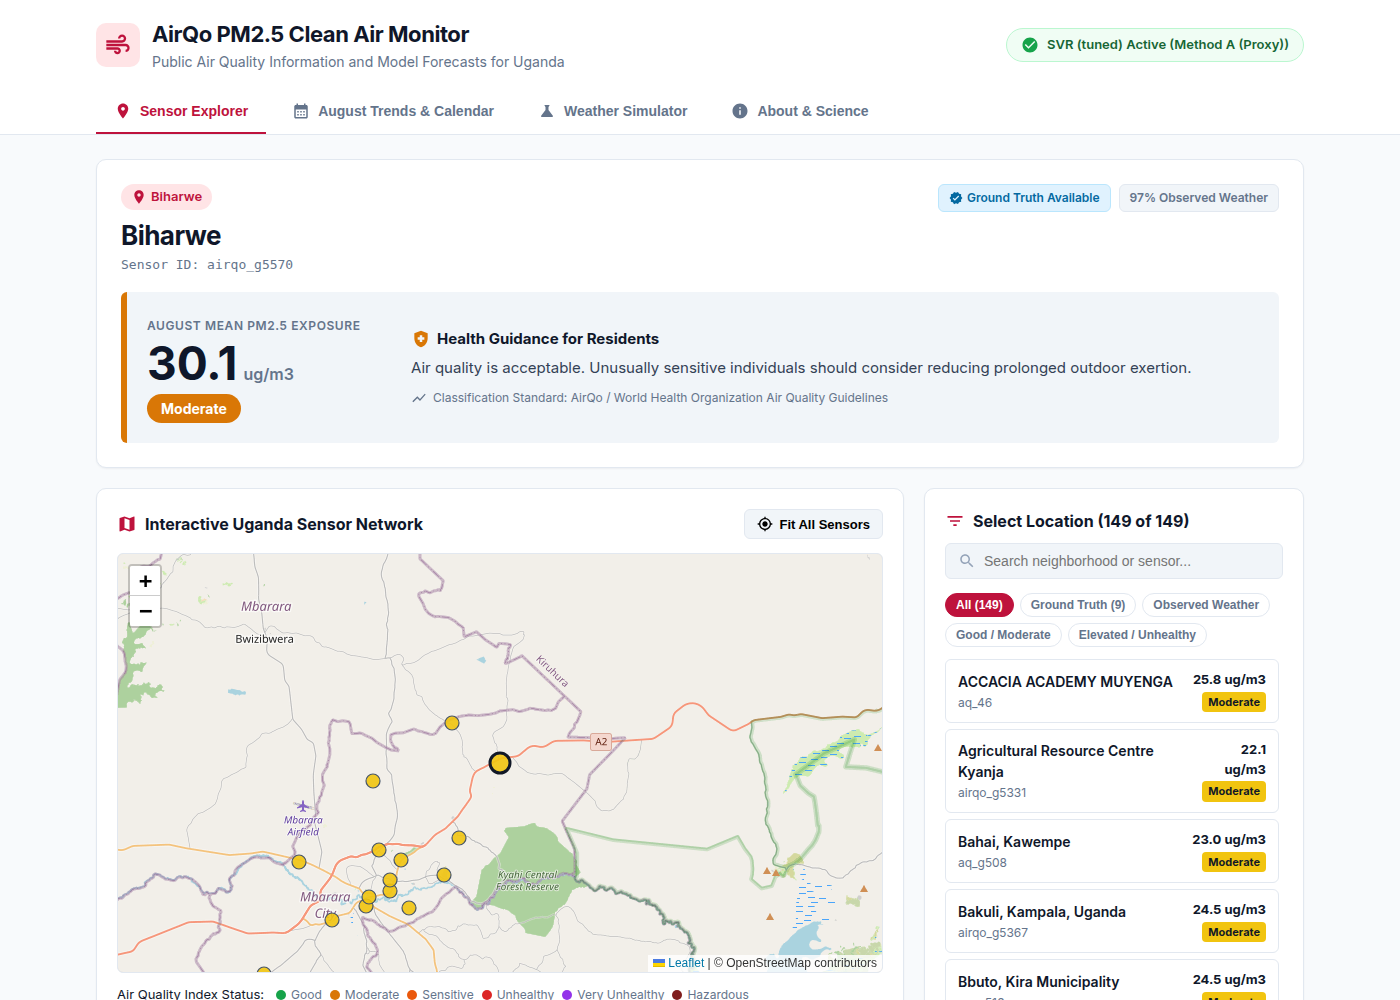
\includegraphics[width=\columnwidth]{dashboard.png}
\caption{The deployed dashboard (Sensor Explorer view), captured on 17 November 2026.}
\label{fig:dashboard}
\end{figure}

\subsection{Remote Access}\label{sec:remote-access}

Getting the model online took four attempts: a GPU rental service needed prepaid credit, a free notebook run did not complete, and a model host refused server-side apps without a paid plan. The fourth put the service on Render and the dashboard on Vercel, which calls the service through a proxy route, falls back to calling Render directly, and warns that a sleeping instance may take a minute to answer.

\section{Results}\label{sec:results}

\subsection{Forecast and Nowcast Accuracy}\label{sec:forecast-and-nowcast-accuracy}

For Objectives 1 and 2, Table~\ref{tab:results} gives each model's error, baselines first. On the hold-out the tuned SVR was the best forecast model, 47\% below the mean baseline, but persistence was better still: 51\% below the mean baseline and 8\% below the SVR (difference 0.76~\ugm{}, 95\% CI 0.15 to 1.34). PM2.5 history lowered the MAE of the random forest by 12\% and of LightGBM by 14\%, and raised $R^2$ from about 0.25 to 0.42, but beat persistence by only 1--2\%, a difference whose interval includes zero (LightGBM with history: $-$0.15~\ugm{}, 95\% CI $-$0.53 to 0.24).

\begin{table*}[t]
\caption{Error of each model (MAE, RMSE in~\ugm{}; best in bold). CI: 95\% sensor bootstrap; CV: expanding-window cross-validation; LSO: leave-sensors-out; RF: random forest. Linear, polynomial and ridge regression (hold-out MAE 22.0--23.9, August 43.1--49.0) and the tuned RF (within 0.2 of the untuned one) are omitted.}
\label{tab:results}
\centering
\scriptsize
\setlength{\tabcolsep}{3pt}
\begin{tabular}{lcccccccccc}
\toprule
 & \multicolumn{3}{c}{Hold-out (2--3 June)} & \multicolumn{2}{c}{Expanding-window CV} & \multicolumn{2}{c}{Leave-sensors-out} & \multicolumn{3}{c}{August 2026 (new month)} \\
\cmidrule(lr){2-4}\cmidrule(lr){5-6}\cmidrule(lr){7-8}\cmidrule(lr){9-11}
Model & MAE$\downarrow$ [95\% CI] & RMSE$\downarrow$ & $R^2\uparrow$ & MAE$\downarrow$ & $R^2\uparrow$ & MAE$\downarrow$ & $R^2\uparrow$ & MAE$\downarrow$ [95\% CI] & RMSE$\downarrow$ & $R^2\uparrow$ \\
\midrule
\multicolumn{11}{l}{\textit{Baselines}} \\
Mean & 17.60 {\scriptsize[16.7, 18.6]} & 21.17 & $-$0.30 & 24.11 & $-$1.08 & 20.33 & $-$0.03 & 19.21 {\scriptsize[18.4, 20.1]} & 26.04 & $-$0.01 \\
Persistence & 8.58 {\scriptsize[7.6, 9.5]} & 16.25 & 0.24 & \textbf{9.53} & 0.20 & 9.46 & 0.56 & 15.17 {\scriptsize[14.0, 16.3]} & 25.02 & 0.07 \\
\midrule
\multicolumn{11}{l}{\textit{Forecast models}} \\
SVR & 9.34 {\scriptsize[8.6, 10.2]} & 15.14 & 0.34 & 14.68 & $-$0.06 & 15.09 & 0.27 & 18.32 {\scriptsize[17.1, 19.6]} & 27.95 & $-$0.16 \\
RF & 9.61 {\scriptsize[8.8, 10.5]} & 16.14 & 0.25 & 27.02 & $-$2.38 & 14.90 & 0.22 & 19.05 {\scriptsize[17.8, 20.5]} & 28.67 & $-$0.22 \\
LightGBM & 9.82 {\scriptsize[9.0, 10.8]} & 16.08 & 0.25 & 27.45 & $-$2.30 & 15.12 & 0.27 & 18.78 {\scriptsize[17.5, 20.1]} & 27.94 & $-$0.16 \\
KNN & 9.62 {\scriptsize[8.7, 10.6]} & 15.62 & 0.29 & 15.69 & $-$0.34 & 16.05 & 0.17 & 19.36 {\scriptsize[18.2, 20.6]} & 28.58 & $-$0.21 \\
LSTM & 12.22 {\scriptsize[11.1, 13.5]} & 18.53 & 0.01 & 20.70 & $-$1.41 & 15.60 & 0.26 & 19.47 {\scriptsize[18.7, 20.3]} & 26.61 & $-$0.05 \\
\midrule
\multicolumn{11}{l}{\textit{Nowcast models}} \\
RF + history & 8.50 {\scriptsize[7.7, 9.3]} & 14.25 & 0.41 & 10.25 & \textbf{0.23} & \textbf{9.03} & 0.65 & \textbf{13.70} {\scriptsize[12.8, 14.5]} & \textbf{21.71} & \textbf{0.30} \\
LightGBM + history & \textbf{8.43} {\scriptsize[7.7, 9.2]} & \textbf{14.21} & \textbf{0.42} & 12.08 & 0.08 & 9.49 & 0.63 & 14.02 {\scriptsize[13.1, 14.8]} & 22.14 & 0.27 \\
LSTM + history & 10.89 {\scriptsize[10.2, 11.7]} & 15.58 & 0.30 & 12.18 & 0.15 & 9.41 & \textbf{0.65} & 19.31 {\scriptsize[18.6, 20.0]} & 25.58 & 0.03 \\
\bottomrule
\end{tabular}
\end{table*}

Fig.~\ref{fig:obspred} shows why errors stay high: the SVR missed every peak, and the history models followed them an hour late. Without history, the random forest and LightGBM placed 46\% and 32\% of their SHAP attribution on the month and only 5--8\% each on temperature and humidity; with six training days in three months, the month mostly tells a model which burst a row came from.

\begin{figure*}[t]
\centering
% Generated by research_paper_draft3/reruns/make_figures_tex.py from review_extras (train.ipynb rerun).
\begin{tikzpicture}
\begin{groupplot}[group style={group size=1 by 2, vertical sep=17mm},
  width=\textwidth, height=40mm, xmin=0, xmax=7, ymin=0, ymax=195, xtick={0,...,7},
  xlabel={Days from start of week}, ylabel={PM2.5 (\ugm)}, label style={font=\scriptsize},
  tick label style={font=\scriptsize}, title style={font=\scriptsize\bfseries, text=pbluedark},
  ymajorgrids, grid style={black!15}, axis x line*=bottom, axis y line*=left, unbounded coords=jump]
\nextgroupplot[legend to name=oplegend, legend columns=4, legend style={font=\scriptsize, draw=none, /tikz/every even column/.append style={column sep=6pt}}, title={Sensor airqo\_g5570 (data-rich), 19--25 August 2026}]
\addplot[black, line width=0.9pt] table[x=day, y=obs, col sep=comma] {figures/data/fig_obspred_1.csv};
\addplot[pblue!45, line width=0.8pt] table[x=day, y=svr, col sep=comma] {figures/data/fig_obspred_1.csv};
\addplot[pbluedark, line width=0.8pt] table[x=day, y=lgbh, col sep=comma] {figures/data/fig_obspred_1.csv};
\addplot[black!45, densely dashed, line width=0.6pt] table[x=day, y=persist, col sep=comma] {figures/data/fig_obspred_1.csv};
\legend{Observed, SVR (forecast model), LightGBM + PM2.5 history, Persistence}
\nextgroupplot[title={Sensor aq\_g530 (intermediate), 12--18 August 2026}]
\addplot[black, line width=0.9pt] table[x=day, y=obs, col sep=comma] {figures/data/fig_obspred_2.csv};
\addplot[pblue!45, line width=0.8pt] table[x=day, y=svr, col sep=comma] {figures/data/fig_obspred_2.csv};
\addplot[pbluedark, line width=0.8pt] table[x=day, y=lgbh, col sep=comma] {figures/data/fig_obspred_2.csv};
\addplot[black!45, densely dashed, line width=0.6pt] table[x=day, y=persist, col sep=comma] {figures/data/fig_obspred_2.csv};
\end{groupplot}
\end{tikzpicture}

\ref{oplegend}

\caption{Observed and predicted PM2.5 in August 2026 at a data-rich (top) and an intermediate sensor (bottom), in the week of each sensor's highest reading.}
\label{fig:obspred}
\end{figure*}

\subsection{Imputation Accuracy and Downstream Effect}\label{sec:imputation-accuracy-and-downstream-effect}

For Objective 3, PM2.5 is assessed too because the BRITS-style model fills all three variables jointly. The bidirectional model beat the time-of-day method in all 15 variable-gap combinations, by 20.8\% on average (Table~\ref{tab:imputation}), and kept its accuracy on August (1.3~\textdegree{}C at six-hour gaps); interpolation was best for short gaps but filled only 618 of 11,423 missing temperatures. Downstream, the effect was not consistent (Table~\ref{tab:downstream}): the bidirectional imputer's weather changed prediction MAE by +1.1\% on average and helped in 3 of 15 cases, against $-$0.4\% and 7 of 15 in the first run, so the final models kept (a) and (b).

\begin{table*}[t]
\caption{Imputation MAE on hidden values: (a) windowed interpolation, (b) time-of-day profile, (c) BRITS-style; best in bold.}
\label{tab:imputation}
\centering
\footnotesize
\begin{tabular}{lllllll}
\toprule
Variable & Method & 1 h & 3 h & 6 h & 12 h & 24 h \\
\midrule
Temp. (\textdegree{}C) & (a) & \textbf{0.49} & \textbf{0.77} & - & - & - \\
 & (b) & 1.61 & 1.71 & 1.87 & 2.06 & 2.13 \\
 & (c) & 0.76 & 1.13 & \textbf{1.36} & \textbf{1.74} & \textbf{1.97} \\
Humidity (\%) & (a) & \textbf{1.80} & \textbf{2.66} & - & - & - \\
 & (b) & 5.91 & 5.94 & 6.76 & 7.40 & 7.99 \\
 & (c) & 2.90 & 4.24 & \textbf{5.67} & \textbf{7.12} & \textbf{7.39} \\
PM2.5 (\ugm{}) & (a) & 7.35 & \textbf{9.29} & - & - & - \\
 & (b) & 9.10 & 10.80 & 10.42 & 10.39 & 12.13 \\
 & (c) & \textbf{6.85} & 9.52 & \textbf{9.80} & \textbf{9.32} & \textbf{10.26} \\
\bottomrule
\end{tabular}
\end{table*}

\begin{table*}[t]
\caption{Prediction MAE (\ugm{}) with weather filled by (a), (b) (final models) or (c); best per design in bold.}
\label{tab:downstream}
\centering
\footnotesize
\begin{tabular}{llllllllll}
\toprule
Model & Hold-out (a) & Hold-out (b) & Hold-out (c) & CV (a) & CV (b) & CV (c) & LSO (a) & LSO (b) & LSO (c) \\
\midrule
SVR & \textbf{9.34} & 9.34 & 9.37 & 16.28 & \textbf{14.68} & 16.51 & 15.09 & \textbf{15.09} & 15.11 \\
LightGBM & 9.94 & \textbf{9.82} & 9.90 & \textbf{26.63} & 27.45 & 27.51 & \textbf{15.12} & 15.12 & 15.14 \\
LightGBM + history & \textbf{8.33} & 8.43 & 8.44 & \textbf{11.85} & 12.08 & 11.95 & 9.48 & 9.49 & \textbf{9.47} \\
LSTM & \textbf{12.17} & 12.22 & 12.34 & 21.59 & \textbf{20.70} & 21.32 & 15.80 & \textbf{15.60} & 15.70 \\
LSTM + history & \textbf{10.20} & 10.89 & 10.95 & 12.16 & 12.18 & \textbf{11.95} & 9.56 & \textbf{9.41} & 9.48 \\
\bottomrule
\end{tabular}
\end{table*}

\subsection{Stability and Transfer to a New Month}\label{sec:stability-and-transfer-to-a-new-month}

For Objective 4, in expanding-window cross-validation the tree-based forecast models were 11--14\% worse than the mean baseline, and persistence beat the history models (Table~\ref{tab:results}). At withheld sensors the random forest with history was 5\% better than persistence, and the forecast models 26\% better than the mean baseline but 60\% worse than persistence.

On August, more polluted than the hold-out days (35.5 against 23~\ugm{}), the non-linear forecast models came within 5\% of the mean baseline with $R^2$ below zero, so they did worse than August's own mean. Only the history models beat persistence: the random forest with history by 10\% ($-$1.47~\ugm{}, 95\% CI $-$1.76 to $-$1.16). The LSTM with history over-predicted by 11.1~\ugm{}. Evidently flagged the month as the most drifted input (0.83), yet holding it constant raised the SVR's August MAE from 18.32 to 20.51~\ugm{}. Neither unfamiliar sensors nor missingness explains the errors: every August sensor was seen in training, and the SVR's error was 18.7, 18.1 and 14.3~\ugm{} at data-rich, intermediate and data-poor sensors. Applying the extreme-value rule to August lowered errors by 0.5--1.0~\ugm{} without changing the ranking.

\subsection{Deployment}\label{sec:deployment}

For Objective 5, Table~\ref{tab:deploy} reports agreement with local predictions, warm latency (median request time once awake), cold-start time and monthly cost. The service agreed on all 2,642 rows; a warm one-row request took 0.6 s, mostly overhead, and the first request after a pause took 42 s, which an always-on instance would remove for USD 7 per month~\cite{ref_render}.

\begin{table}[t]
\caption{The deployed forecast service, measured on 17 November 2026 from a client laptop.}
\label{tab:deploy}
\centering
\footnotesize
\begin{tabularx}{\columnwidth}{>{\raggedright\arraybackslash}X>{\raggedright\arraybackslash}X}
\toprule
Measure & Value \\
\midrule
Model file, forecast / nowcast & 1.2 MB / 0.6 MB \\
Local prediction, 1 / 3,576 rows & 3.2 ms / 0.54 s \\
Hosted request, 1 / 100 / 1,000 rows (medians) & 0.56 / 0.70 / 2.51 s \\
First request after spin-down & 41.9 s (one measurement) \\
Agreement with local predictions & 2,642 of 2,642 rows \\
Hosting cost per month & USD 0 free; USD 7 always on \\
\bottomrule
\end{tabularx}
\end{table}

\subsection{Additional Findings}\label{sec:additional-findings}

\textbf{A misleadingly accurate first model.} The first random forest, given PM10, reached an MAE of 3.10~\ugm{}, but PM10 carried about 76\% of its importance, and forecasting August with typical PM10 values merely repeated each site's daily pattern. \textbf{Oversampling.} SMOTE made all eight models tried worse (LightGBM: 9.82 to 29.31~\ugm{} at 0.25). \textbf{Sensitivity.} The index category is a weak yardstick (SVR 75.2\% correct against 74.4\% for the mean). Scoring against untouched readings raised every MAE by about 1.3~\ugm{}, and dropping rows with PM2.5 above PM10 made the hold-out worse (SVR 10.51~\ugm{}).

\section{Business Benefits}\label{sec:business}

The intended users are network operators such as AirQo, city authorities who need early warning of polluted hours, and developers building on low-cost networks. Costs are low: both parts run on free tiers~\cite{ref_render,ref32}, and an always-on service would cost USD 7 per month. Sustainability needs a live feed with an hourly ingestion job for a nowcast, and retraining as continuous data accumulate.

The demonstrated impact is modest, as no users have evaluated the service yet. We propose a three-month pilot with the Kampala Capital City Authority (KCCA) or a school, connecting the nowcast to 10--20 live sensors and judging it by its MAE against persistence, the share of hours at or above 35.5~\ugm{} it flags and whether users changed any decision. No such pilot has been agreed.

\section{Discussion}\label{sec:discussion}

On Objectives 1 and 2, a model without PM2.5 history learns from a few days only each burst's and sensor's level, which did not carry over. The history models were the most stable, but persistence matched them on the hold-out and beat them in cross-validation, so most of their value lies in the last reading itself. Weather mattered little here, as it did over three years in Kampala, where meteorology explained about 18\% of PM2.5 variation~\cite{ref35}. Niyonzima et al.~\cite{ref10} reported an MAE of 8.71~\ugm{} on 759,480 AirQo hours, of the same order as our 8.43~\ugm{} in a different design.

On Objective 3, the best gap-filler did not help because weather carries little of the attribution, and SMOTE failed because oversampling polluted hours raised the level the models learned, whereas the test days were cleaner (23 against 33~\ugm{}). On Objective 4, a possible explanation for the LSTM's August failure, not tested here, is that August's month encoding lies outside the training months, along which a neural network extrapolates and a random forest cannot; since removing the month hurt, the deeper problem is a record too short to show change between months. 

The limitations are substantial: eight days in three bursts, a 28-hour hold-out, one network mostly in Kampala, sensor error (including the 23\% of rows with PM2.5 above PM10), possibly real episodes among the replaced extremes, and confidence intervals that ignore the run-to-run variation the second run revealed, so differences of a few percent are not a ranking.

\subsection{Lessons Learned}\label{sec:lessons-learned}

\textbf{1. Compare with persistence, not only the mean.} Against the mean, the history models looked 52\% better; against persistence, 1--2\%.

\textbf{2. Suspect an excellent score.} The PM10 model's 3.10~\ugm{} came from a co-measurement of the target.

\textbf{3. Test out of period.} Forecast models that scored 9.6--9.8~\ugm{} on the hold-out were worse than the mean in cross-validation.

\textbf{4. Judge imputation by its effect on the task.} A 20.8\% better gap-filler did not improve prediction.

\textbf{5. Rerun on a second machine.} It exposed a tuning near-tie and run-to-run variation before submission.

\section{Conclusions and Summary Recommendations}\label{sec:conclusions}

We built, evaluated and deployed an hourly PM2.5 predictor from eight days of low-cost sensor readings. Weather-only models came within 5\% of a mean baseline on a later month; models with three hours of PM2.5 history matched persistence on the hold-out and beat it by 10\% in August; better imputation and oversampling did not help; and the forecast model runs at no cost. Such data support SDG indicator 11.6.2 and target 3.9~\cite{ref22,ref23}.

\textbf{Network operators (for example AirQo)} should report persistence beside nowcasts and keep sensors online in long runs. \textbf{Researchers and developers} should use out-of-period tests, exclude co-measured pollutants and compare with persistence. \textbf{City authorities (for example KCCA)} should base alerts on live nowcasts, piloted against a clear measure (Section~\ref{sec:business}); for unmonitored places, our forecast models cut the mean baseline's error by about a quarter at withheld sensors, but new sensors would do more for policy than any model trained on so short a record.

Future work should retrain on continuous data, test the LSTM's August failure, add multi-step forecasting and neighbouring sensors, and automate drift monitoring and retraining. On this record, the best guide to the next hour's PM2.5 was the last hour's reading.

\section*{Data and Code Availability}

\ifblind AirQo data are available from AirQo under CC BY 4.0~\cite{ref29}; the code and outputs are in a public repository, withheld for review.\else AirQo data are available from AirQo under CC BY 4.0~\cite{ref29}; the code and outputs are at \url{https://github.com/coleRodneyMigisha/airqo_cole_charis_assgnmnt}.\fi

\section*{Acknowledgment}

\ifblind Acknowledgements are withheld for double-blind review.\else The authors thank AirQo, Makerere University, for access to its air quality monitoring data, used under CC BY 4.0, and acknowledge AirGradient as an originating data provider.\fi

\section*{Declaration of use of content generated by Artificial Intelligence (AI) (including but not limited to Generative-AI) in the paper}

The authors acknowledge the use of content generated by Artificial Intelligence (AI) (including but not limited to text, figures, images, and code) in the paper entitled ``\papertitle'' in the following ways:

The research questions, data processing, analysis, model and deployment decisions, findings and conclusions are the authors' own, recorded in the project's notebook and report. Claude (Anthropic), through Claude Code, assisted with parts of the analysis code; drafted text, tables and figures from the authors' report, notebook outputs and cited sources; and, in revising the paper after the supervisor's review, wrote and ran the additional analyses the review asked for and checked the references. The authors reviewed, revised and verified the content and take full responsibility for it.

\bibliographystyle{IEEEtran}
\bibliography{references}

\EOD
\end{document}
